\documentclass[11pt]{article} 
\usepackage[english]{babel}
\usepackage[utf8]{inputenc}
\usepackage[margin=0.5in]{geometry}
\usepackage{amsmath}
\usepackage{amsthm}
\usepackage{amsfonts}
\usepackage{amssymb}
\usepackage[usenames,dvipsnames]{xcolor}
\usepackage{graphicx}
\usepackage[siunitx]{circuitikz}
\usepackage{tikz}
\usepackage[colorinlistoftodos, color=orange!50]{todonotes}
\usepackage{hyperref}
\usepackage[numbers, square]{natbib}
\usepackage{fancybox}
\usepackage{epsfig}
\usepackage{soul}
\usepackage[framemethod=tikz]{mdframed}
\usetikzlibrary{positioning, automata, backgrounds}
\usepackage[shortlabels]{enumitem}
\usepackage[version=4]{mhchem}
\usepackage{multicol}
\usepackage{forest}
\usepackage{mathtools}
\usepackage{comment}
\usepackage{enumitem}
\usepackage[utf8]{inputenc}
\usepackage[linesnumbered,ruled,vlined]{algorithm2e}
\usepackage{listings}
\usepackage{color}
\usepackage[numbers]{natbib}
\usepackage{subfiles}
\usepackage{tkz-berge}


\newtheorem{prop}{Proposition}[section]
\newtheorem{thm}{Theorem}[section]
\newtheorem{lemma}{Lemma}[section]
\newtheorem{cor}{Corollary}[prop]

\theoremstyle{definition}
\newtheorem{definition}{Definition}

\theoremstyle{definition}
\newtheorem{required}{Problem}

\theoremstyle{definition}
\newtheorem{ex}{Example}

\newcommand{\interval}[4]{\draw (#2, #1) -- (#3, #1); % Usage: \interval{height}{start}{end}{label}
\draw (#2, #1-0.11) -- (#2, #1+0.11); % draw left whisker
\draw (#3, #1-0.11) -- (#3, #1+0.11); % draw right whisker
\node[] at (#2-0.25, #1) {#4};
}

\setlength{\marginparwidth}{3.4cm}
%#########################################################

%To use symbols for footnotes
\renewcommand*{\thefootnote}{\fnsymbol{footnote}}
%To change footnotes back to numbers uncomment the following line
%\renewcommand*{\thefootnote}{\arabic{footnote}}

% Enable this command to adjust line spacing for inline math equations.
% \everymath{\displaystyle}

% _______ _____ _______ _      ______ 
%|__   __|_   _|__   __| |    |  ____|
%   | |    | |    | |  | |    | |__   
%   | |    | |    | |  | |    |  __|  
%   | |   _| |_   | |  | |____| |____ 
%   |_|  |_____|  |_|  |______|______|
%%%%%%%%%%%%%%%%%%%%%%%%%%%%%%%%%%%%%%%

\title{
\normalfont \normalsize 
\textsc{CSCI 3104 Spring 2022 \\ 
Instructors: Profs. Chen and Layer} \\
[10pt] 
\rule{\linewidth}{0.5pt} \\[6pt] 
\huge Problem Set 2 \\
\rule{\linewidth}{2pt}  \\[10pt]
}
%\author{}
\date{}

\begin{document}

\definecolor {processblue}{cmyk}{0.96,0,0,0}
\definecolor{processred}{rgb}{200, 0, 0}
\definecolor{processgreen}{rgb}{0, 255, 0}
\DeclareGraphicsExtensions{.png}
\DeclareGraphicsExtensions{.gif}
\DeclareGraphicsExtensions{.jpg}

\maketitle


%%%%%%%%%%%%%%%%%%%%%%%%%
%%%%%%%%%%%%%%%%%%%%%%%%%%
%%%%%%%%%%FILL IN YOUR NAME%%%%%%%
%%%%%%%%%%AND STUDENT ID%%%%%%%%
%%%%%%%%%%%%%%%%%%%%%%%%%%
\noindent
Due Date \dotfill February 1, 2022 \\
Name \dotfill \textbf{Your Name} \\
Student ID \dotfill \textbf{Your Student ID} \\
Collaborators \dotfill \textbf{List Your Collaborators Here}

\tableofcontents

\section{Instructions}
 \begin{itemize}
	\item The solutions \textbf{should be typed}, using proper mathematical notation. We cannot accept hand-written solutions. \href{http://ece.uprm.edu/~caceros/latex/introduction.pdf}{Here's a short intro to \LaTeX.}
	\item You should submit your work through the \textbf{class Canvas page} only. Please submit one PDF file, compiled using this \LaTeX \ template.
	\item You may not need a full page for your solutions; pagebreaks are there to help Gradescope automatically find where each problem is. Even if you do not attempt every problem, please submit this document with no fewer pages than the blank template (or Gradescope has issues with it).

	\item You are welcome and encouraged to collaborate with your classmates, as well as consult outside resources. You must \textbf{cite your sources in this document.} \textbf{Copying from any source is an Honor Code violation. Furthermore, all submissions must be in your own words and reflect your understanding of the material.} If there is any confusion about this policy, it is your responsibility to clarify before the due date. 

	\item Posting to \textbf{any} service including, but not limited to Chegg, Reddit, StackExchange, etc., for help on an assignment is a violation of the Honor Code.

	\item You \textbf{must} virtually sign the Honor Code (see Section \ref{HonorCode}). Failure to do so will result in your assignment not being graded.
\end{itemize}


\section{Honor Code (Make Sure to Virtually Sign)} \label{HonorCode}

\begin{required}
\begin{itemize}
\item My submission is in my own words and reflects my understanding of the material.
\item Any collaborations and external sources have been clearly cited in this document.
\item I have not posted to external services including, but not limited to Chegg, Reddit, StackExchange, etc.
\item I have neither copied nor provided others solutions they can copy.
\end{itemize}

%\noindent In the specified region below, clearly indicate that you have upheld the Honor Code. Then type your name. 
\end{required}

\begin{proof}[Agreed (signature here).]
%% Typing "I agree to the above," followed by your name is sufficient.
I agree to the above, Chengming Li
\end{proof}


%%%%%%%%%%%%%%%%%%%%%%%%%%%%%%%%%%%%%%%%%%%%%%%%%%
\newpage
\section{Standard 5- BFS and DFS}
\subsection{Problem \ref{DFS1}}
\begin{required} \label{DFS1}
Consider a \textsf{Modified Connectivity} problem:
\begin{itemize}
\item \textsf{Instance:} Let $G(V, E)$ be a simple, undirected graph. Let $s, t \in V(G)$.
\item \textsf{Decision:} Given an integer $k\geq 1$,  is there a shortest path from $s$ to $t$ in $G$ that consists of $k$ edges? Here the length/weight of a path is defined as the number of edges of the path. 
\end{itemize}

\noindent \\ Do the following. [\textbf{Note:} There are parts (a) and (b). Part (b) is on the next page.]
\begin{enumerate}[label=(\alph*)]
\item Design an algorithm to solve the $\textsf{Modified Connectivity}$ problem. Your solution should provide enough detail that a CSCI 2270 student could reasonably be expected to implement your solution.
\begin{proof}[Answer for Part (a)]

%Your answer goes here
The way to solve finding the shortest path from s to t in G is using the algorithm of BFS.
\begin{itemize}
\item The main concept is that visiting all of the unvisited neighbors of the current node before visiting further away.
\item Each node in the graph should at least have following components: neighbor, visited-status, prev-node.

\item (1) This algorithm should create an empty set, Q(queue), which used to stored the visited nodes in the future and traverse the graph based on the first item in the Q. Moreover, the nodes will be placed in the queue, but they will also be removed from the queue when the algorithm is in the process.

\item (2)The first node will be placed in the Q is $s$ and its status will be marked as visited, its prev-node should be initialized to $NULL$.

\item (3)The algorithm will jump into a $while$ loop, and will end until the Q is an empty set, or queue.
\item (4)At the beginning of each iteration, the first item in the Q will be polled from the Q, and then stored in a temporary variable, $current$. Then there is another $for$ loop after that. The $for$ loop will visited every unvisited neighbor node of $current$. In the order words, the algorithm will never visit the visited neighbor node again.
\item (5)Once the algorithm jump into the current $for$ loop, the algorithm should mark each unvisited neighbor node as $visited$, and put those unvisited neighbor of $current$ node into Q.
\item (6)Inside the $for$ loop, the algorithm will always check if we hit the target node $t$. If it is the target node, the algorithm will break the $while$ loop. 
\item (7) If it is not the target node, the current $for$ iteration should finish, the program will jump back to the $while$ loop to check whether the condition, Q is not an empty set, still hold. If it still holds , repeated the step$(4)-(7)$ as stated above.
\item (8) The shortest path can be found by back-traversed the prev-node of target node, because the shortest path is connected by the prev-node element from $t$ back to $s$.

\end{itemize}
\end{proof}



\newpage
\item We say that the graph $G$ is \textit{connected} if for every pair of vertices $s, t \in V(G)$, there exists a path from $s$ to $t$. Design an algorithm to determine whether $G$ is connected. Your algorithm should only traverse the graph once - this means that you should \textbf{not} apply BFS or DFS more than once. Your solution should provide enough detail that a CSCI 2270 student could reasonably be expected to implement your solution.

\begin{proof}[Answer for Part (b)]
%Your answer goes here
The algorithm to solve this problem is using DFS to traverse the graph.
\begin{itemize}
\item The main concept to check if the graph is connected is making sure every node in the graph has been visited.
\item For every node in the graph, they should at least have the following components: name, visited-status.
\item (1) The DFS algorithm takes two input, Graph G and Vertex s. At the beginning of the function,the algorithm mark the current input Vertex s as visited.
\item (2) Then, the function will traverse every unvisited neighbor node, $v$ of $s$ using $for$ loop.
\item (3) Inside the $for$ loop, the algorithm will recursive call the $DFS$ function itself with 2 input arguments, Graph G and Vertex $v$.
\item (4) The algorithm will repeat $step(1)-(3)$ until there is no more unvisited neighbor node v of s in the graph. And the DFS algorithm function is finished.
\item (5)Last,we should check the status of each node in the graph to see whether it has been visited. If every node in the graph has been visited, the conclusion is the graph G is connected. However, if there is node has not been visited, the conclusion is the graph G is not connected because there must be exist a pair of vertices $s,t\in V(G)$ that doesn't exist a path between them.


\end{itemize}
\end{proof}
\end{enumerate}
\end{required}






\newpage
\subsection{Problem \ref{DFS2}} 
\begin{required} \label{DFS2}
Give an example of a simple, undirected, and unweighted graph $G(V, E)$ that has a single source shortest path tree which a \textbf{depth-first traversal} will not return for any ordering of its vertices. 
    Your answer must
    \begin{enumerate}[label=(\alph*)]
    	\item Provide a drawing of the graph $G$. [\textbf{Note:} We have provided TikZ code below if you wish to use \LaTeX \ to draw the graph. Alternatively, you may hand-draw $G$ and embed it as an image below, provided that (i) your drawing is legible and (ii) we do not have to rotate our screens to grade your work.]
    	\item Specify the single source shortest path tree $T = (V,E_T)$ by specifying $E_T$ and also specifying the root $s \in V$. [\textbf{Note:} You may again hand-draw this tree. If you wish, you may clearly mark the edges of $T$ on your drawing of $G$. Please make it easy on the graders to identify the edges of $T$.] 
    	\item Include a clear explanation of why the depth-first search algorithm we discussed in class will never produce $T$ for any orderings of the vertices.
    \end{enumerate}

\end{required}

\noindent 
\begin{proof}[Answer]
%Your proof goes here.
\noindent \textbf{Part a)}
\begin{center}
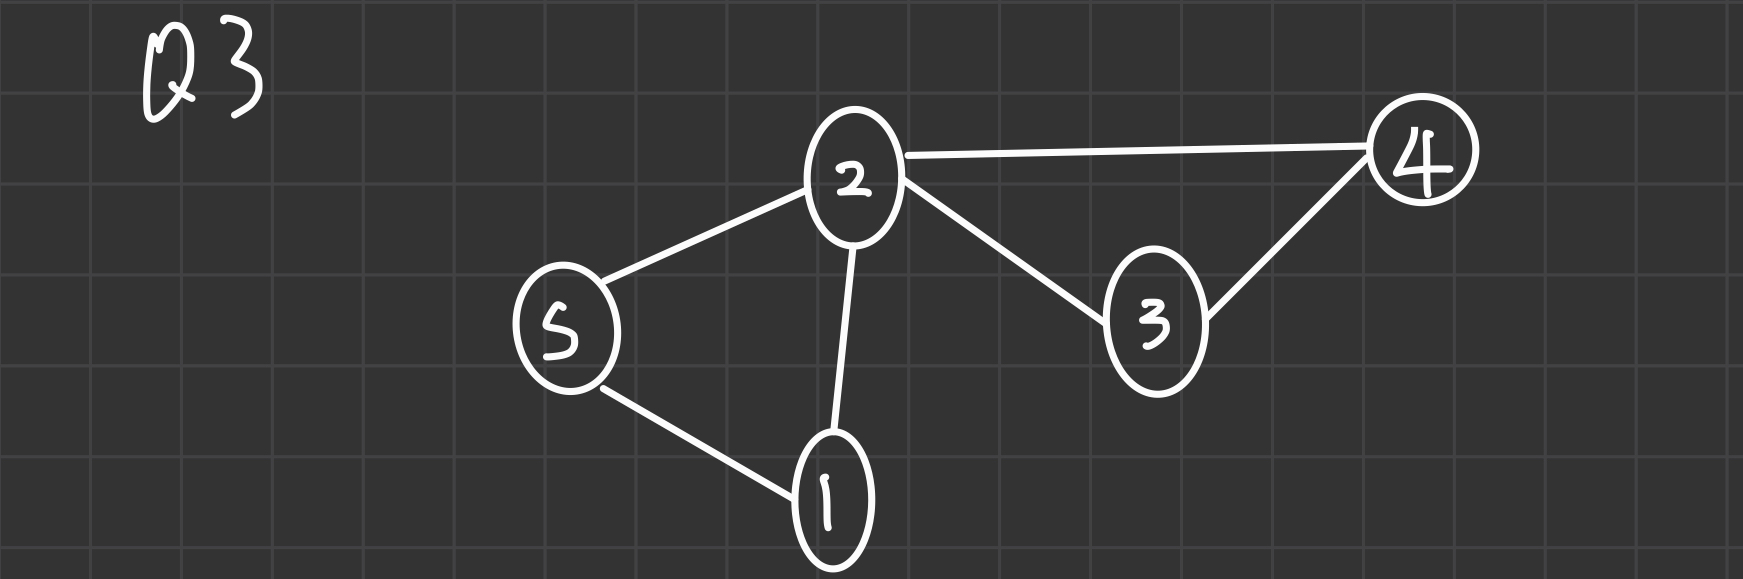
\includegraphics[width=0.5\textwidth]{Q3A.PNG}
\end{center}

\noindent \textbf{Part b)}
\begin{center}
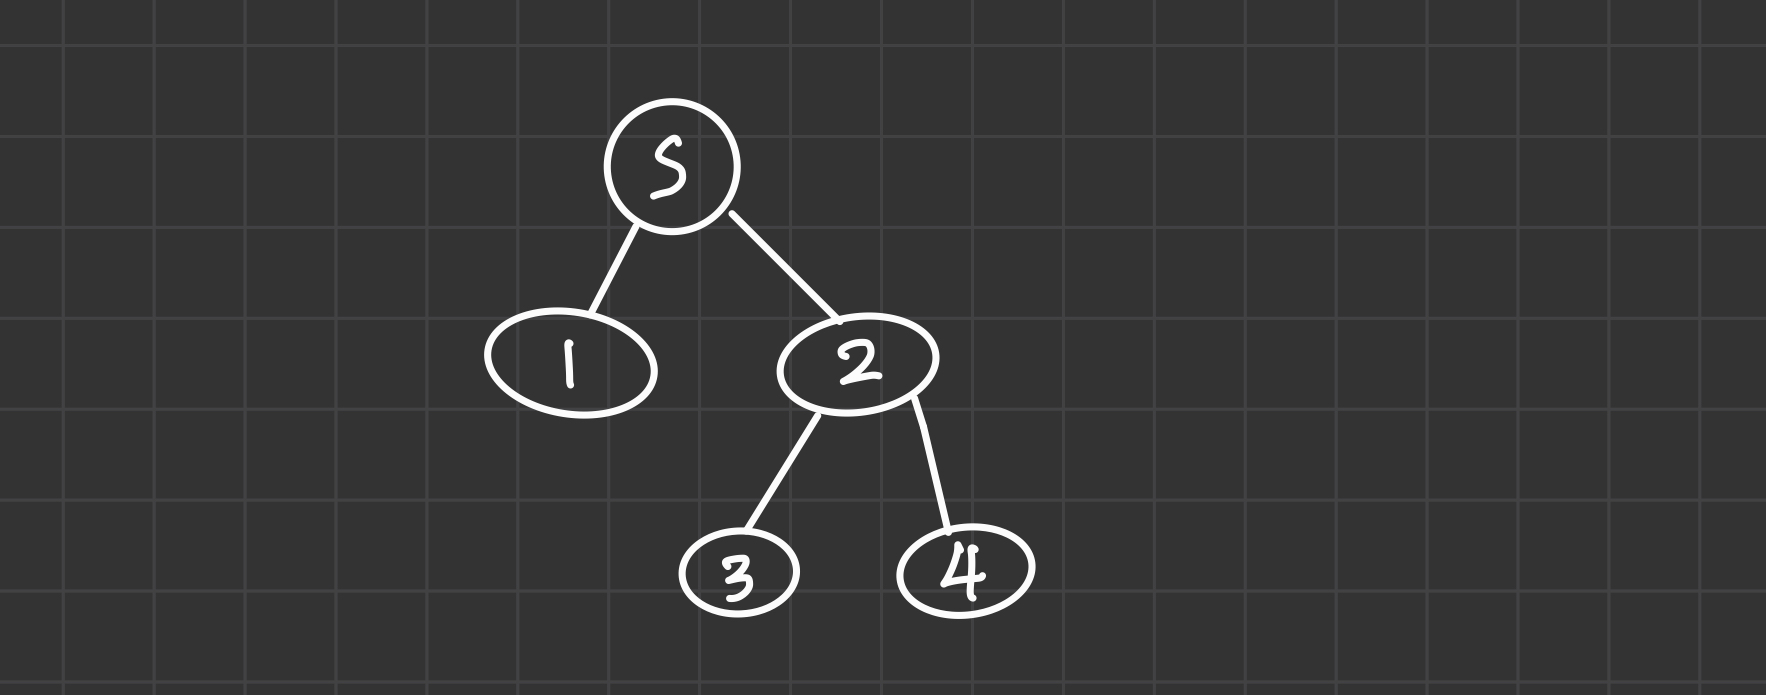
\includegraphics[width=0.5\textwidth]{Q3B.PNG}
\end{center}
\noindent \textbf{Part c)}
By the DFS, the single source shortest path tree will never produce T that seen in Part b), because the DFS algorithm will recursively traverse the unvisited neighbors of s  until there is no more unvisited neighbors, or reach the dead-end. Even two vertices at the same depth of T will have different length from the tree. The DFS algorithm will traverse some unnecessary path to get to a specific vertex, which make the path from s to t is not the shortest.\\
In the order words, DFS algorithm aims to find the path as deep as possible first from the source vertex $s$ even if there exist another way to hit the target vertex $t$. Moreover, the DFS algorithm will not end the recursion if it find the shortest path to a vertex $t$. The only condition to terminate the algorithm to produce tree is the dead-end is reached (i.e., a node whose neighbors have all be explored). \\
Here are a few example trees that produced by DFS based on the Graph in Part a):\\
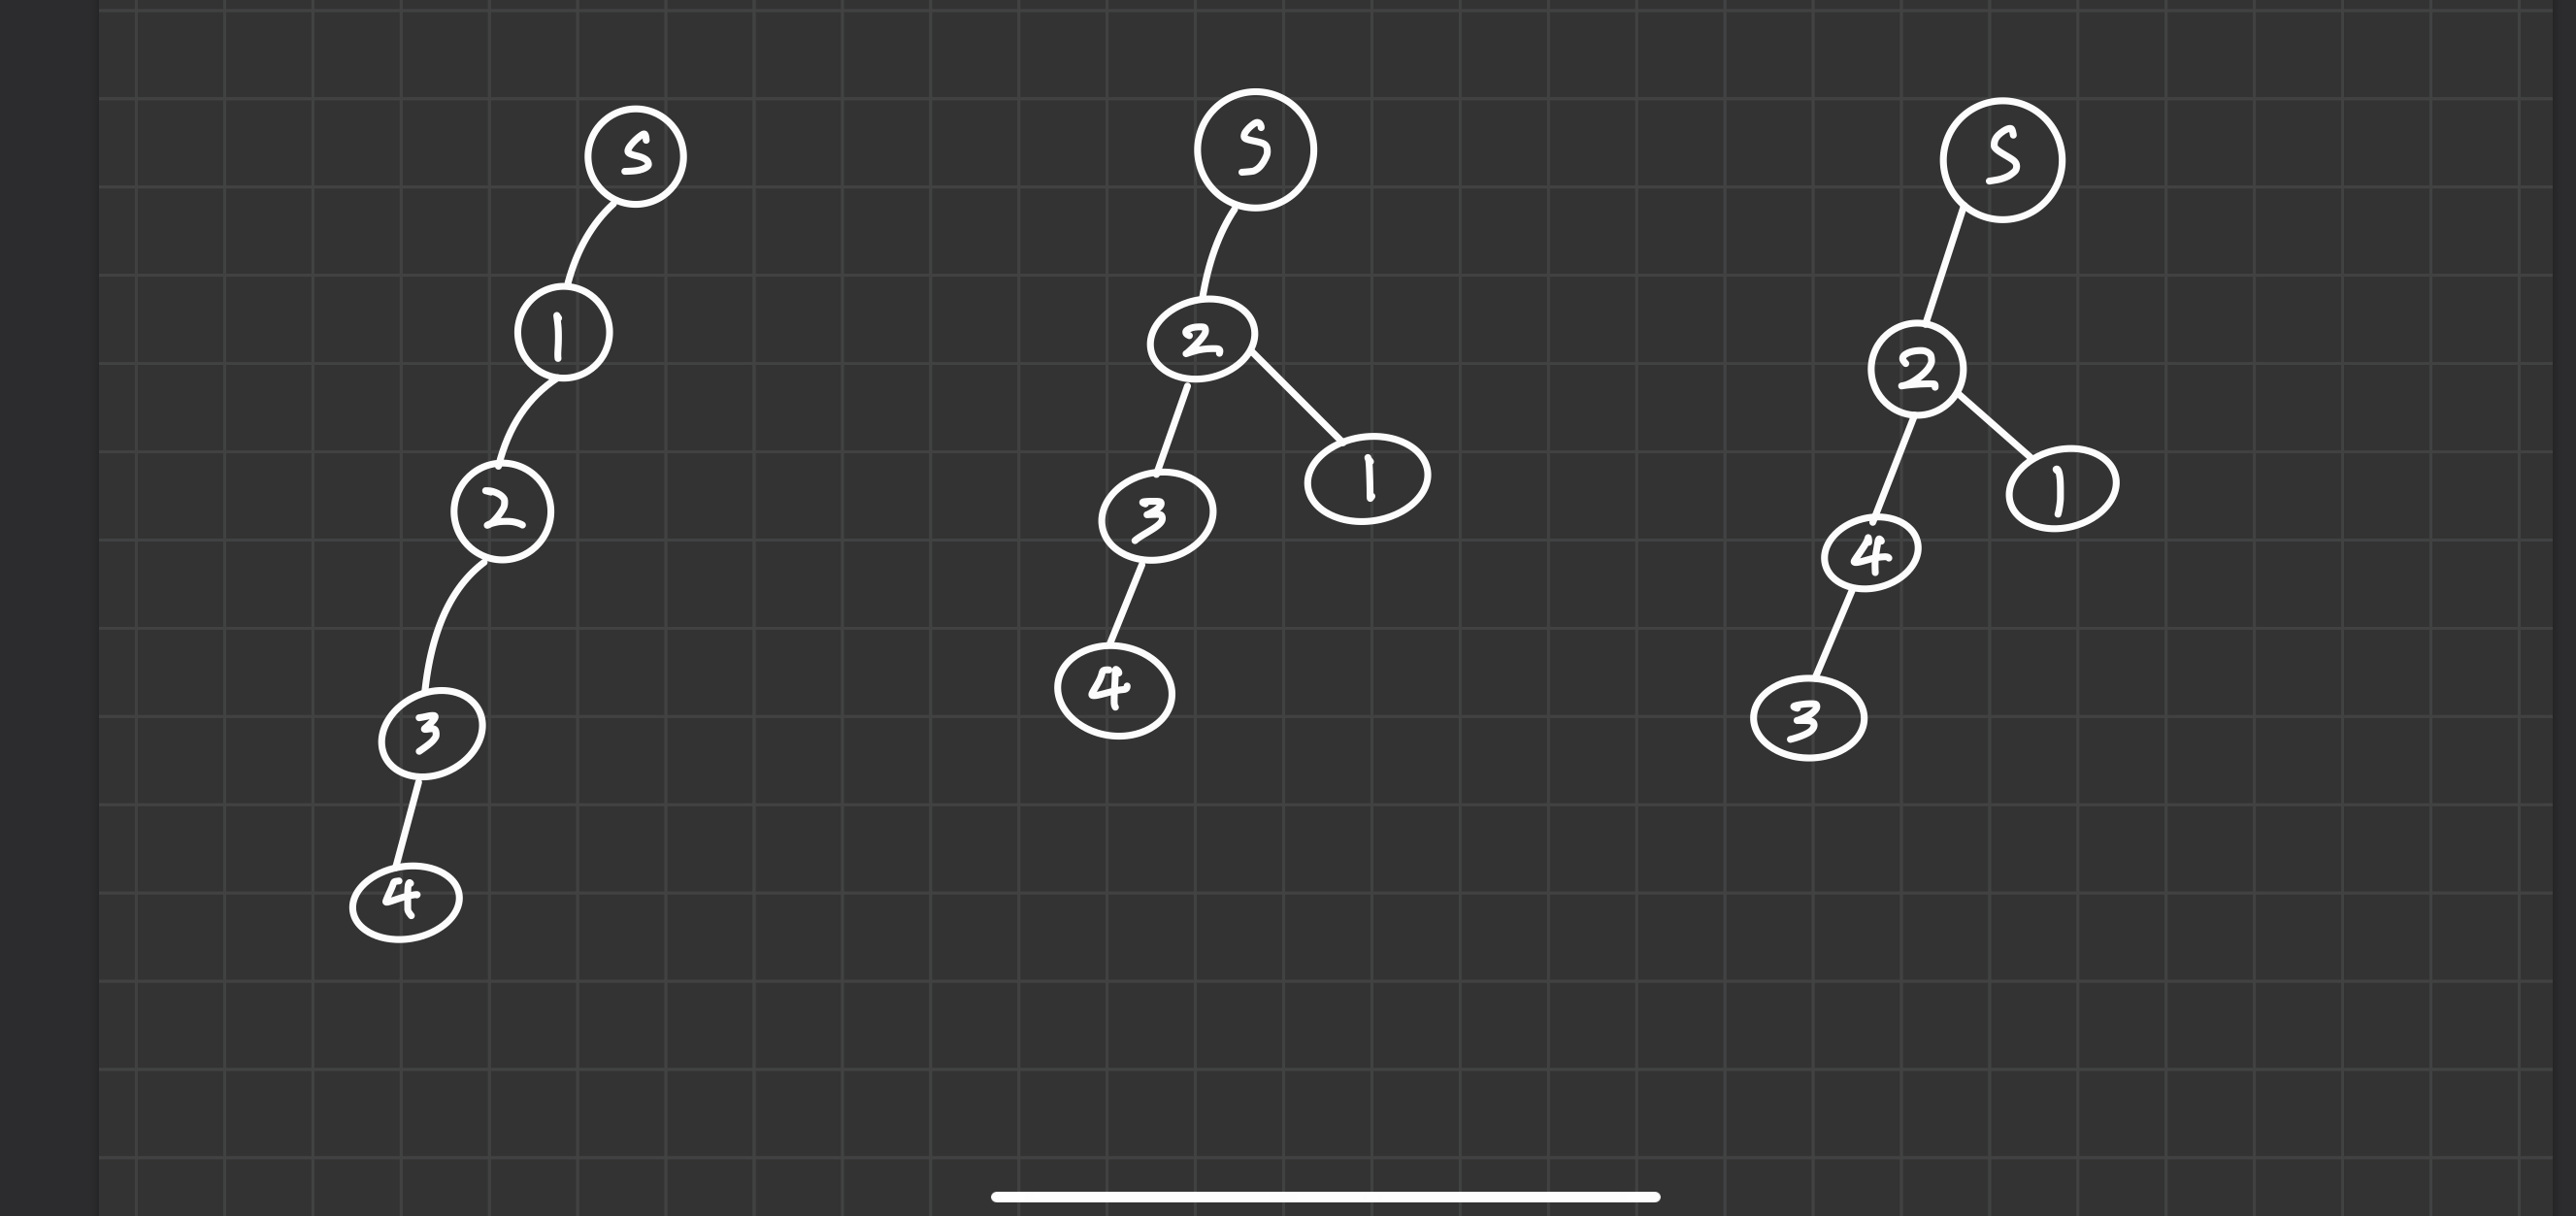
\includegraphics[width=0.5\textwidth]{Q3C.PNG}
\end{proof}









\newpage
\subsection{Problem \ref{DFS4}}
\begin{required} \label{DFS4}
	Give an example of a simple, undirected, weighted graph such that a breadth-first traversal outputs a search-tree that is not a single source shortest path tree. (That is, BFS is not sufficiently powerful to solve the shortest-path problem on weighted graphs. This motivates Dijkstra's algorithm.) 
	Your answer must
	\begin{enumerate}[label=(\alph*)]
		\item Draw the graph $G = (V,E, w)$ by specifying $V$ and $E$, clearly labeling the edge weights.  [\textbf{Note:} We have provided TikZ code below if you wish to use \LaTeX \ to draw the graph. Alternatively, you may hand-draw $G$ and embed it as an image below, provided that (i) your drawing is legible and (ii) we do not have to rotate our screens to grade your work.]
		\item Specify a spanning tree $T(V, E_{T})$ that is returned by BFS, but is not a single-source shortest path tree. [\textbf{Note:} You may again hand-draw this tree. If you wish, you may clearly mark the edges of $T$ on your drawing of $G$. Please make it easy on the graders to identify the edges of $T$.] 

		\item Specify a valid single-source shortest path tree $T^{\prime} = (V,E_{T^{\prime}})$.  [\textbf{Note:} You may again hand-draw this tree. If you wish, you may clearly mark the edges of $T$ on your drawing of $G$. Please make it easy on the graders to identify the edges of $T$.] 

		\item Include a clear explanation of why the search-tree output by breadth-first search is not a valid single-source shortest path tree of $G$.
	\end{enumerate}
\end{required}


\begin{proof}[Answer]
%Your answer here.
\noindent \textbf{Part a)}
\begin{center}
	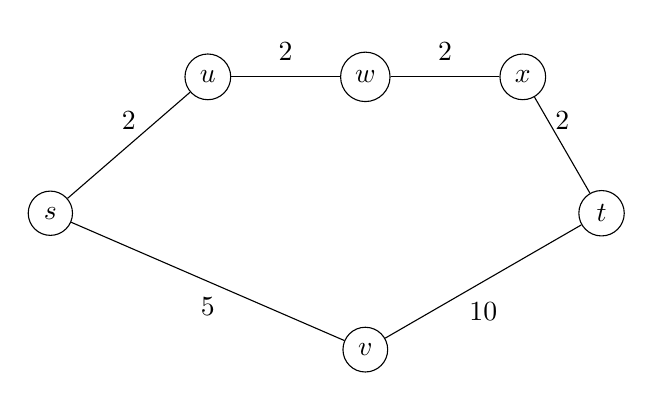
\begin{tikzpicture}[
		wide/.style={line width=4pt},
		every node/.style={circle,draw,minimum size=16},
		scale=2]
		\node (s) at (-0.5,0)            {$s$};
		\node (u) at ($ (0,0) + ( 60:1)$) {$u$};
		\node (v) at ($ (0,0) + (-60:1)+(1,0)$) {$v$};
		\node (w) at ($ (u) + ( 1,0 )$) {$w$};
		\node (x) at ($ (w) + ( 1,0 ) $) {$x$};
		\node (t) at ($ (w) + (-60:1) + (1,0)$) {$t$};


% Replace the line \draw (w) -- (t); with the line below (after deleting the % symbol to uncomment) in order to draw a thicker edge.
%		\draw[line width=3pt] (w) -- (t);


		\draw (s) -- node[below, draw=none,fill=none]{5} (v);
		\draw (v) -- node[below, draw=none,fill=none]{10} (t); 	
		\draw (s) -- node[above, draw=none,fill=none]{2} (u);
		\draw (u) -- node[above, draw=none,fill=none]{2} (w);
		\draw (w) -- node[above, draw=none,fill=none]{2} (x);
		\draw (x) -- node[above, draw=none,fill=none]{2} (t);		
\end{tikzpicture}
\end{center}
\noindent \textbf{Part b)}
\begin{center}
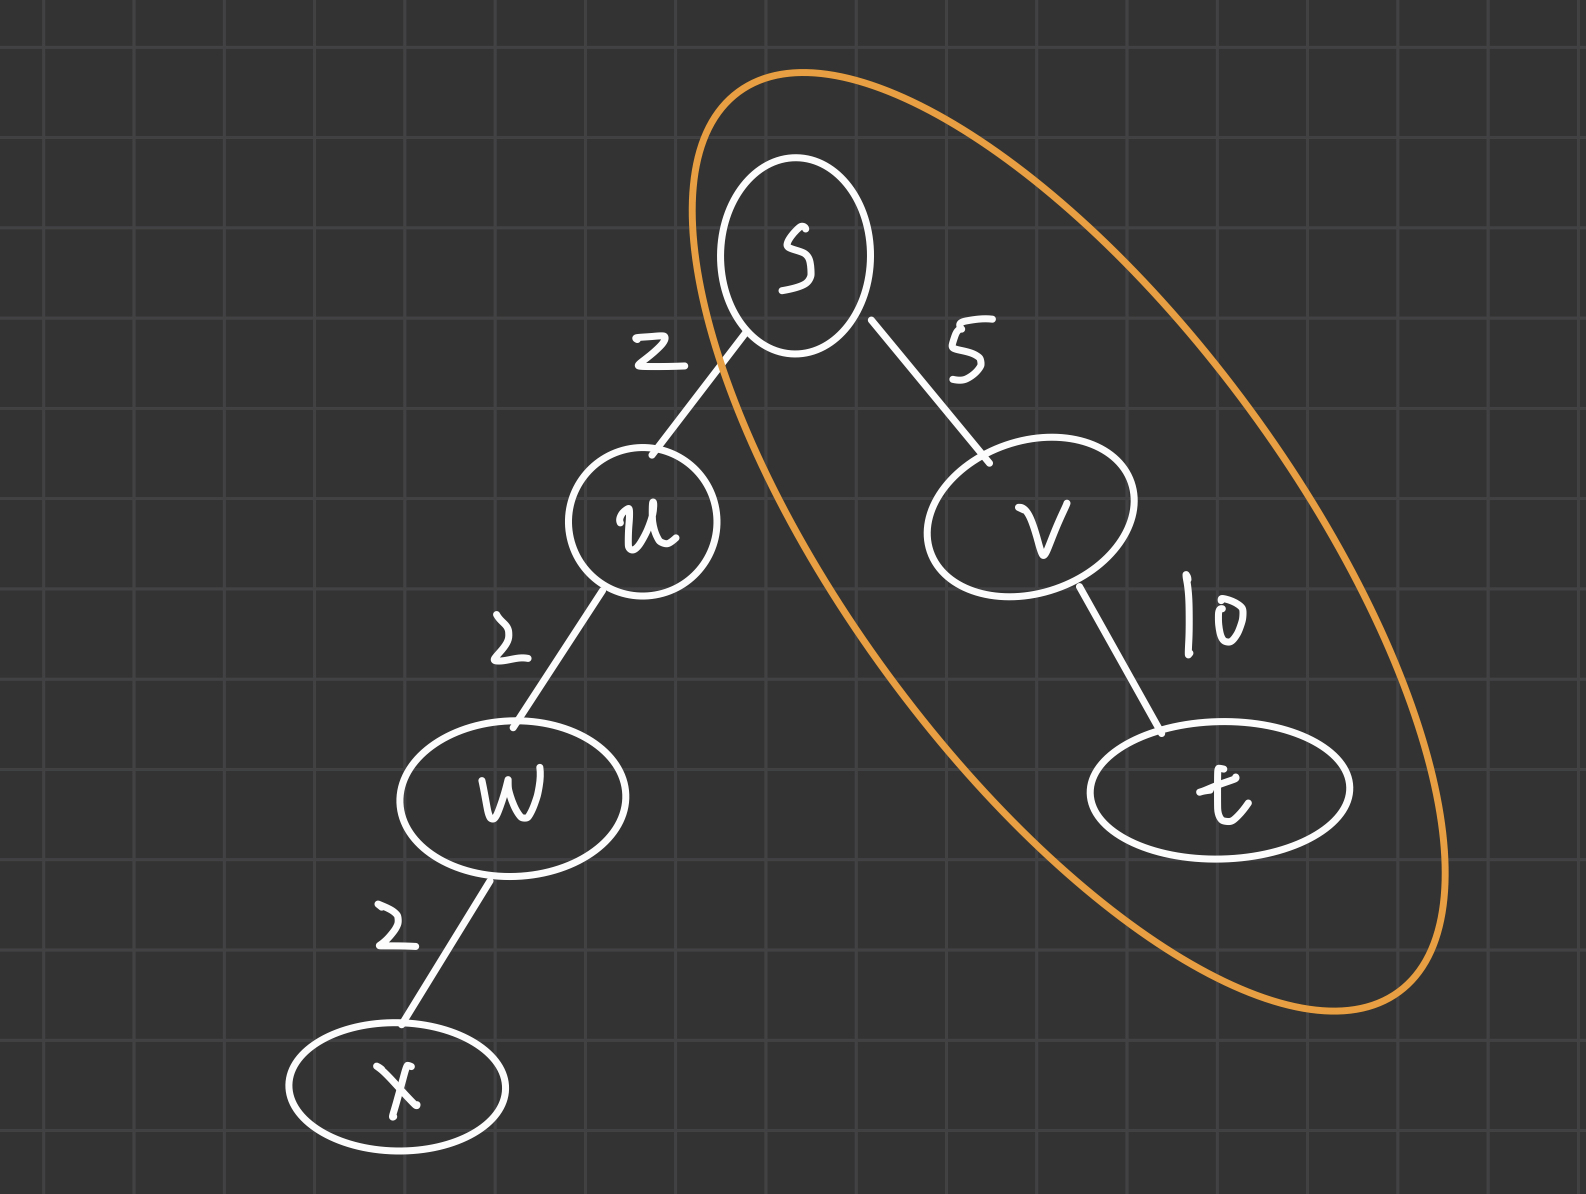
\includegraphics[width=0.5\textwidth]{Q4B.PNG}
\end{center}
\noindent \textbf{Part c)}
\begin{center}
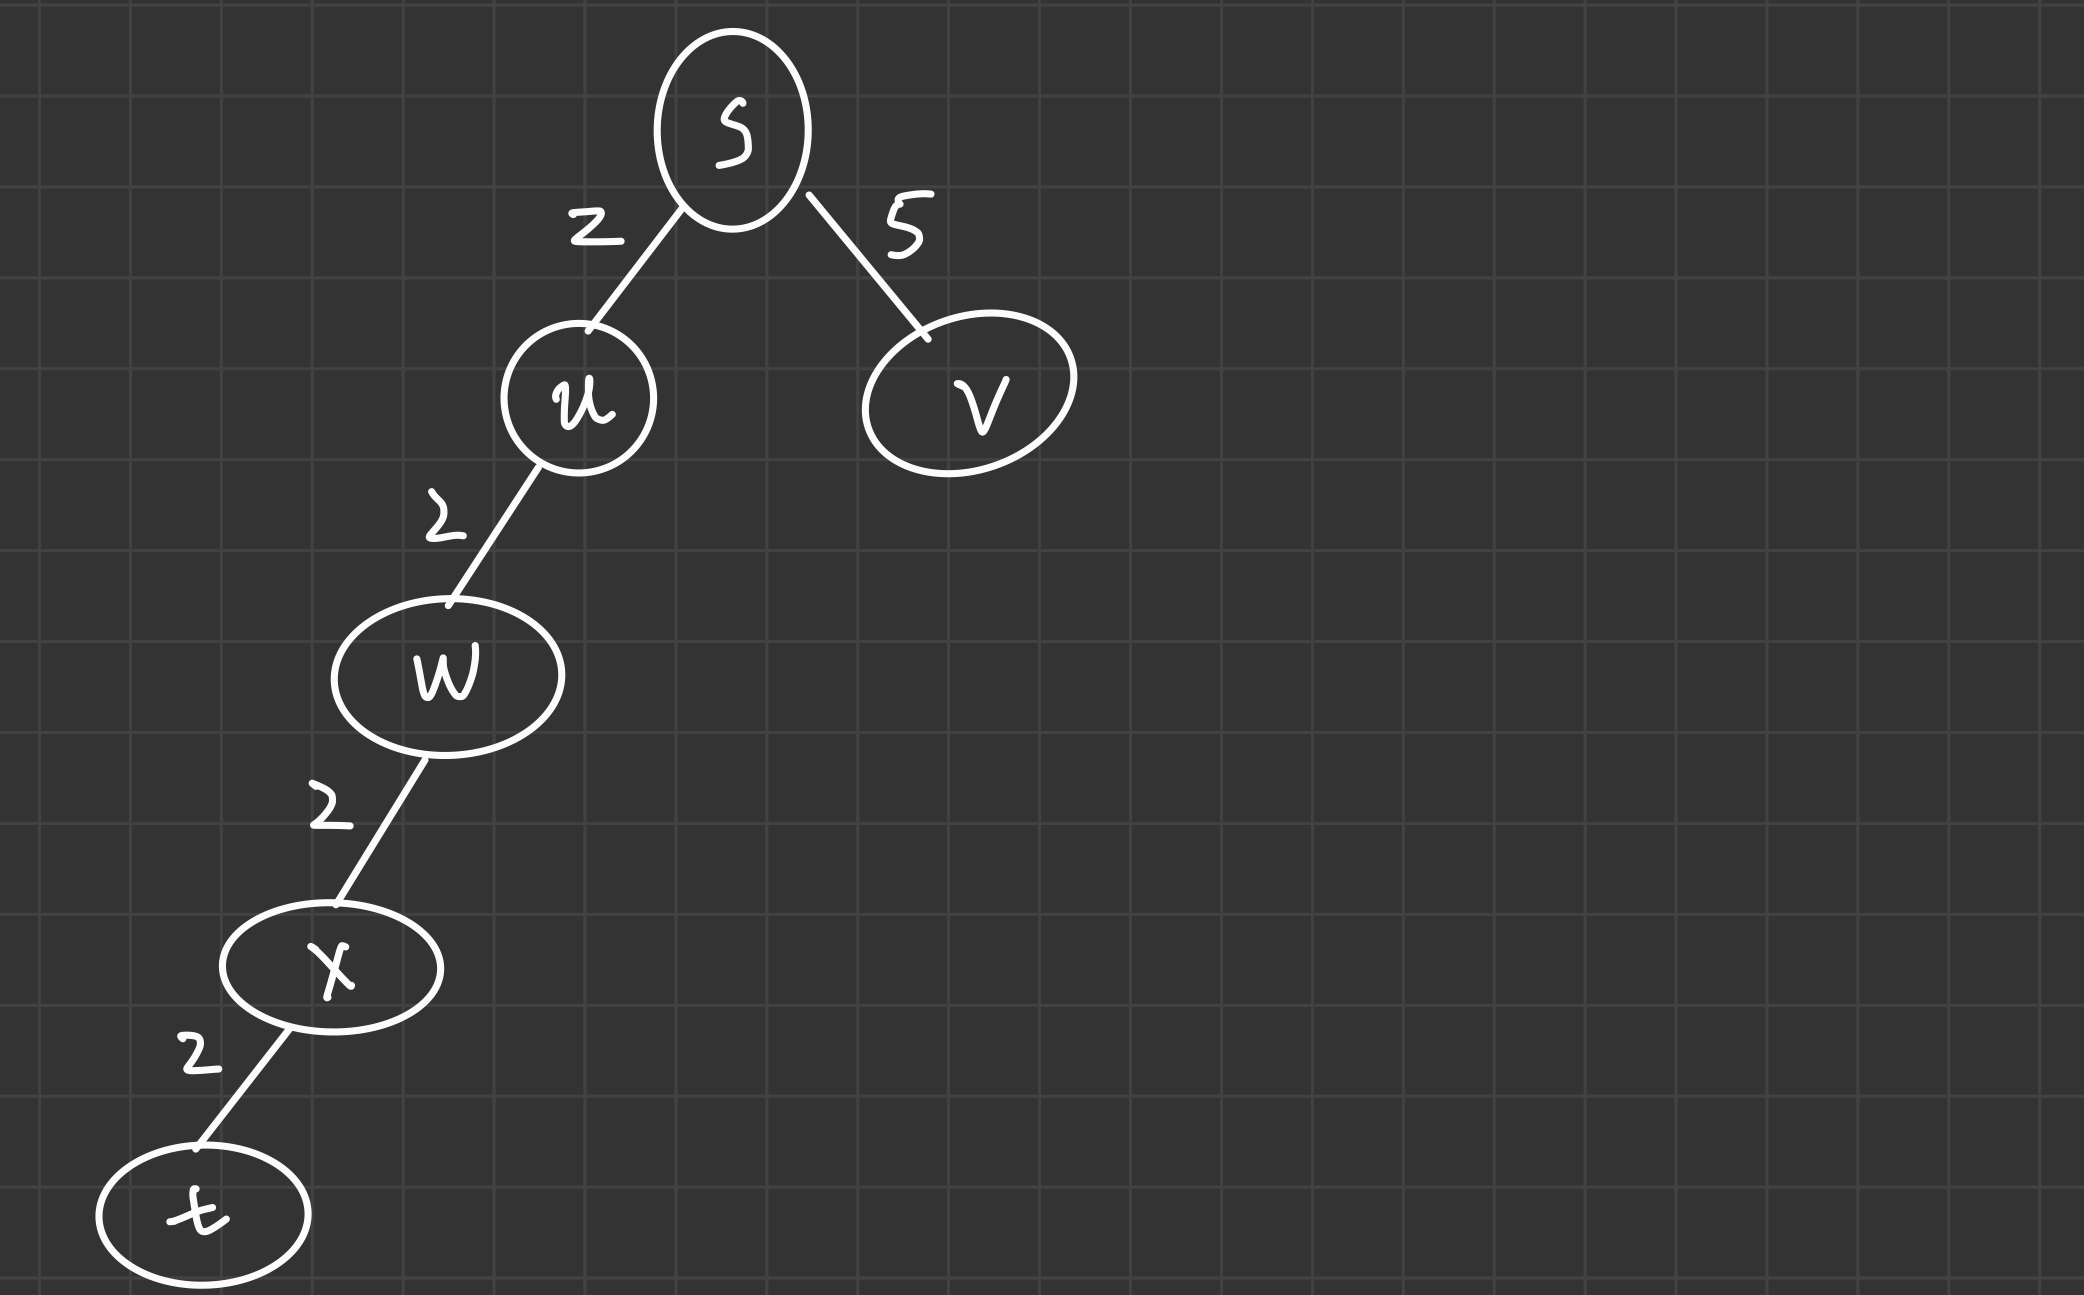
\includegraphics[width=0.5\textwidth]{Q4C.PNG}
\end{center}
\noindent \textbf{Part d)}
By breadth-first search tree, the graph shown in above will not generate a valid single-source shortest path tree of G. Because, the path $s->v->t$ with weight = 15 will hit the vertex, $t$ earlier than the path $s->u->w->x$ with weight = 8. And since the path $s->v->t with weight =15$ find the target vertex, $t$, earlier, it will break the loop and finish the function so that single-source shortest path tree $T^{\prime} = (V,E_{T^{\prime}})$ wouldn't be able to found it by the BFS. 
The changing of queue in BFS at each iteration can be seen below:
\begin{itemize}
\item Q = $\{s\}$
\item Q = $\{u,v\}$
\item Q = $\{v,w\}$
\item Q = $\{w,t\}$
\item Iteration break due to target vertex $t$ has been found. And the spanning tree $T(V, E_{T})$ that is returned by BFS is not a single-source shortest path tree, ie.the path $s->v->t$ with weight = 15 will be returned by BFS.
\end{itemize}
\end{proof}


%%%%%%%%%%%%%%%%%%%%%%%%%%%%%%%%%%%%%%%%%%%%%%%%%%


\newpage
\section{Standard 6- Dijkstra's Algorithm}

\subsection{Problem \ref{Dijkstra0}}
\begin{required} \label{Dijkstra0}
Consider the weighted graph $G(V, E, w)$ pictured below. Work through Dijkstra's algorithm on the following graph, using the source vertex $E$. 
\begin{itemize}
\item Clearly include the contents of the priority queue, as well as the distance from $E$ to each vertex at each iteration.
\item If you use a table to store the distances, clearly label the keys according to the vertex names rather than numeric indices (i.e., \texttt{dist[`B']} is more descriptive than \texttt{dist[`1']}).
\item You do \textbf{not} need to draw the graph at each iteration, though you are welcome to do so. [This may be helpful scratch work, which you do not need to include.]
\end{itemize}


\begin{center}
\begin {tikzpicture}[-latex, auto, node distance =2 cm and 3cm, semithick]
\tikzstyle{blue}=[circle ,top color =white , bottom color = processblue!20 ,draw,processblue , text=blue , minimum width =1 cm];
\tikzstyle{red}=[circle ,top color =white , bottom color = processred!20 ,draw, processred , text=blue , minimum width =1 cm];
\tikzstyle{green}=[circle ,top color =white , bottom color = processgreen!20 ,draw, processgreen , text=blue , minimum width =1 cm];

	\node[blue] (A) {$A$};
	\node[blue] (C) [below right = of A] {$C$};
	\node[blue] (B) [below right = of C] {$B$};
	\node[blue] (E) [below left = of A] {$E$};
	\node[blue] (D) [below left = of E] {$D$};
	\node[blue] (H) [below right = of D] {$H$};
	\node[blue] (F) [right = of H] {$F$};

	\path (A) edge node[above] {$4$} (C);
	\path[line width=3pt] (E) edge node[left] {$9$} (A);

	\path[line width=3pt] (C) edge node[above] {$3$} (B);
	\path (B) edge node[below] {$6$} (F);

	\path[line width=3pt] (E) edge node[above] {$10$} (C);
	\path[line width=3pt] (C) edge node[above] {$2$} (F);

	\path[line width=3pt] (D) edge node[above] {$4$} (H);

	\path (E) edge node[above] {$20$} (F);
	\path[line width=3pt] (E) edge node[right] {$9$} (D);
	\end{tikzpicture}  
\end{center}

\end{required}

\begin{proof}[Answer]

\begin{center}
\begin{tabular}[c]{|c|c|c|} 
	Vertex &Dist from E &Prev-Vertex \\\hline
	A &$\infty$ & NULL\\
	B &$\infty$ & NULL\\
	C &$\infty$& NULL\\
	D &$\infty$ & NULL\\
	E & 0& NULL\\
	F &$\infty$ & NULL\\
	H &$\infty$ & NULL\\
\end{tabular}
\end{center}	
\textbf{PQ = [(E,0)]}

\begin{center}
\begin{tabular}[c]{|c|c|c|} 
	Vertex &Dist from E &Prev-Vertex \\\hline
	A & 9  & E\\
	B &$\infty$ & NULL\\
	C & 10 & E\\
	D &9 & E\\
	E & 0& NULL\\
	F &20 & E\\
	H &$\infty$ & NULL\\
\end{tabular}

\end{center}	
\textbf{PQ = [(A,9),(D,9),(C,10),(F,20)]}
%Your answer here
\begin{center}
\begin{tabular}[c]{|c|c|c|} 
	Vertex &Dist from E &Prev-Vertex \\\hline
	A & 9  & E\\
	B &$\infty$ & NULL\\
	C & 10 & E\\
	D &9 & E\\
	E & 0& NULL\\
	F &20 & E\\
	H &$\infty$ & NULL\\
\end{tabular}
\end{center}	
\textbf{PQ = [(D,9),(C,10),(F,20)]}

\begin{center}
\begin{tabular}[c]{|c|c|c|} 
	Vertex &Dist from E &Prev-Vertex \\\hline
	A & 9  & E\\
	B &$\infty$ & NULL\\
	C & 10 & E\\
	D &9 & E\\
	E & 0& NULL\\
	F &20 & E\\
	H &13 & D\\
\end{tabular}
\end{center}	
\textbf{PQ = [(C,10),(F,20),(H,13)]}

\begin{center}
\begin{tabular}[c]{|c|c|c|} 
	Vertex &Dist from E &Prev-Vertex \\\hline
	A & 9  & E\\
	B &13 & C\\
	C & 10 & E\\
	D &9 & E\\
	E & 0& NULL\\
	F &12 & C\\
	H &13 & D\\
\end{tabular}
\end{center}	
\textbf{PQ = [(F,12),(H,13),(B,13)]}

\begin{center}
\begin{tabular}[c]{|c|c|c|} 
	Vertex &Dist from E &Prev-Vertex \\\hline
	A & 9  & E\\
	B &13 & C\\
	C & 10 & E\\
	D &9 & E\\
	E & 0& NULL\\
	F &12 & C\\
	H &13 & D\\
\end{tabular}
\end{center}	
\textbf{PQ = [(H,13),(B,13)]}

\begin{center}
\begin{tabular}[c]{|c|c|c|} 
	Vertex &Dist from E &Prev-Vertex \\\hline
	A & 9  & E\\
	B &13 & C\\
	C & 10 & E\\
	D &9 & E\\
	E & 0& NULL\\
	F &12 & C\\
	H &13 & D\\
\end{tabular}
\end{center}	
\textbf{PQ = [(B,13)]}

\begin{center}
\begin{tabular}[c]{|c|c|c|} 
	Vertex &Dist from E &Prev-Vertex \\\hline
	A & 9  & E\\
	B &13 & C\\
	C & 10 & E\\
	D &9 & E\\
	E & 0& NULL\\
	F &12 & C\\
	H &13 & D\\
\end{tabular}
\end{center}	
\textbf{PQ = [ ] Algorithm terminates}

\end{proof}





\newpage
\subsection{Problem \ref{Dijkstra2}} 
\begin{required} \label{Dijkstra2}
You have three batteries, with capacities of 40, 25, and 16 Ah (Amp-hours), respectively. The 25 and 16-Ah batteries are fully charged (containing 25 Ah and 16 Ah, respectively), while the 40-Ah battery is empty, with 0 Ah. You have a battery transfer device which has a ``source'' battery position and a ``target'' battery position. When you place two batteries in the device, it instantaneously transfers as many Ah from the source battery to the target battery as possible. Thus, this device stops the transfer either when the source battery has no Ah remaining or when the destination battery is fully charged (whichever comes first).  \\

\noindent But battery transfers aren't free! The battery device is also hooked up to your phone by bluetooth, and automatically charges you a number of dollars equal to however many Ah it just transfered.  \\
	
\noindent The goal in this problem is to determine whether there exists a sequence of transfers that leaves exactly 10 Ah either in the 25-Ah battery or the 16-Ah battery, and if so, how little money you can spend to get this result. \\

\noindent Do the following.
\begin{enumerate}[label=(\alph*)]
\subsubsection{Problem 6\ref{Dijkstra2a}}
\item \label{Dijkstra2a} Rephrase this is as a graph problem. Give a precise definition of how to model this problem as a graph, and state the specific question about this graph that must be answered. [\textbf{Note:} While you are welcome to draw the graph, it is enough to provide 1-2 sentences clearly describing what the vertices are and when two vertices are adjacent. If the graph is weighted, clearly specify what the edge weights are.]

\begin{proof}[Answer]
%Your answer goes here.
\begin{itemize}
\item In the graph, source node can be defined$(0,25,16)$ as 40Ah battery has 0Ah, 25Ah battery has 25Ah and 16Ah battery has 16Ah. And target node can be defined$(15,10,16)$ as  40Ah battery has 15Ah, 25Ah battery has 10Ah and 16Ah battery has 16Ah
\item Each node contains the power left in each battery, there would be three values in each node. And Each node should also contains an element that stores the information of visited status.
\item The edge weights can be considered as the cost of number of dollars, or the Ah it just transfered between two vertices.
\item When there is a transfer between two vertices, we could consider it as two vertices are adjacent.
\item The question can be considered as finding the shortest path from source node to target node.
\item The Graph can be seen below: 
\end{itemize}
\begin{center}
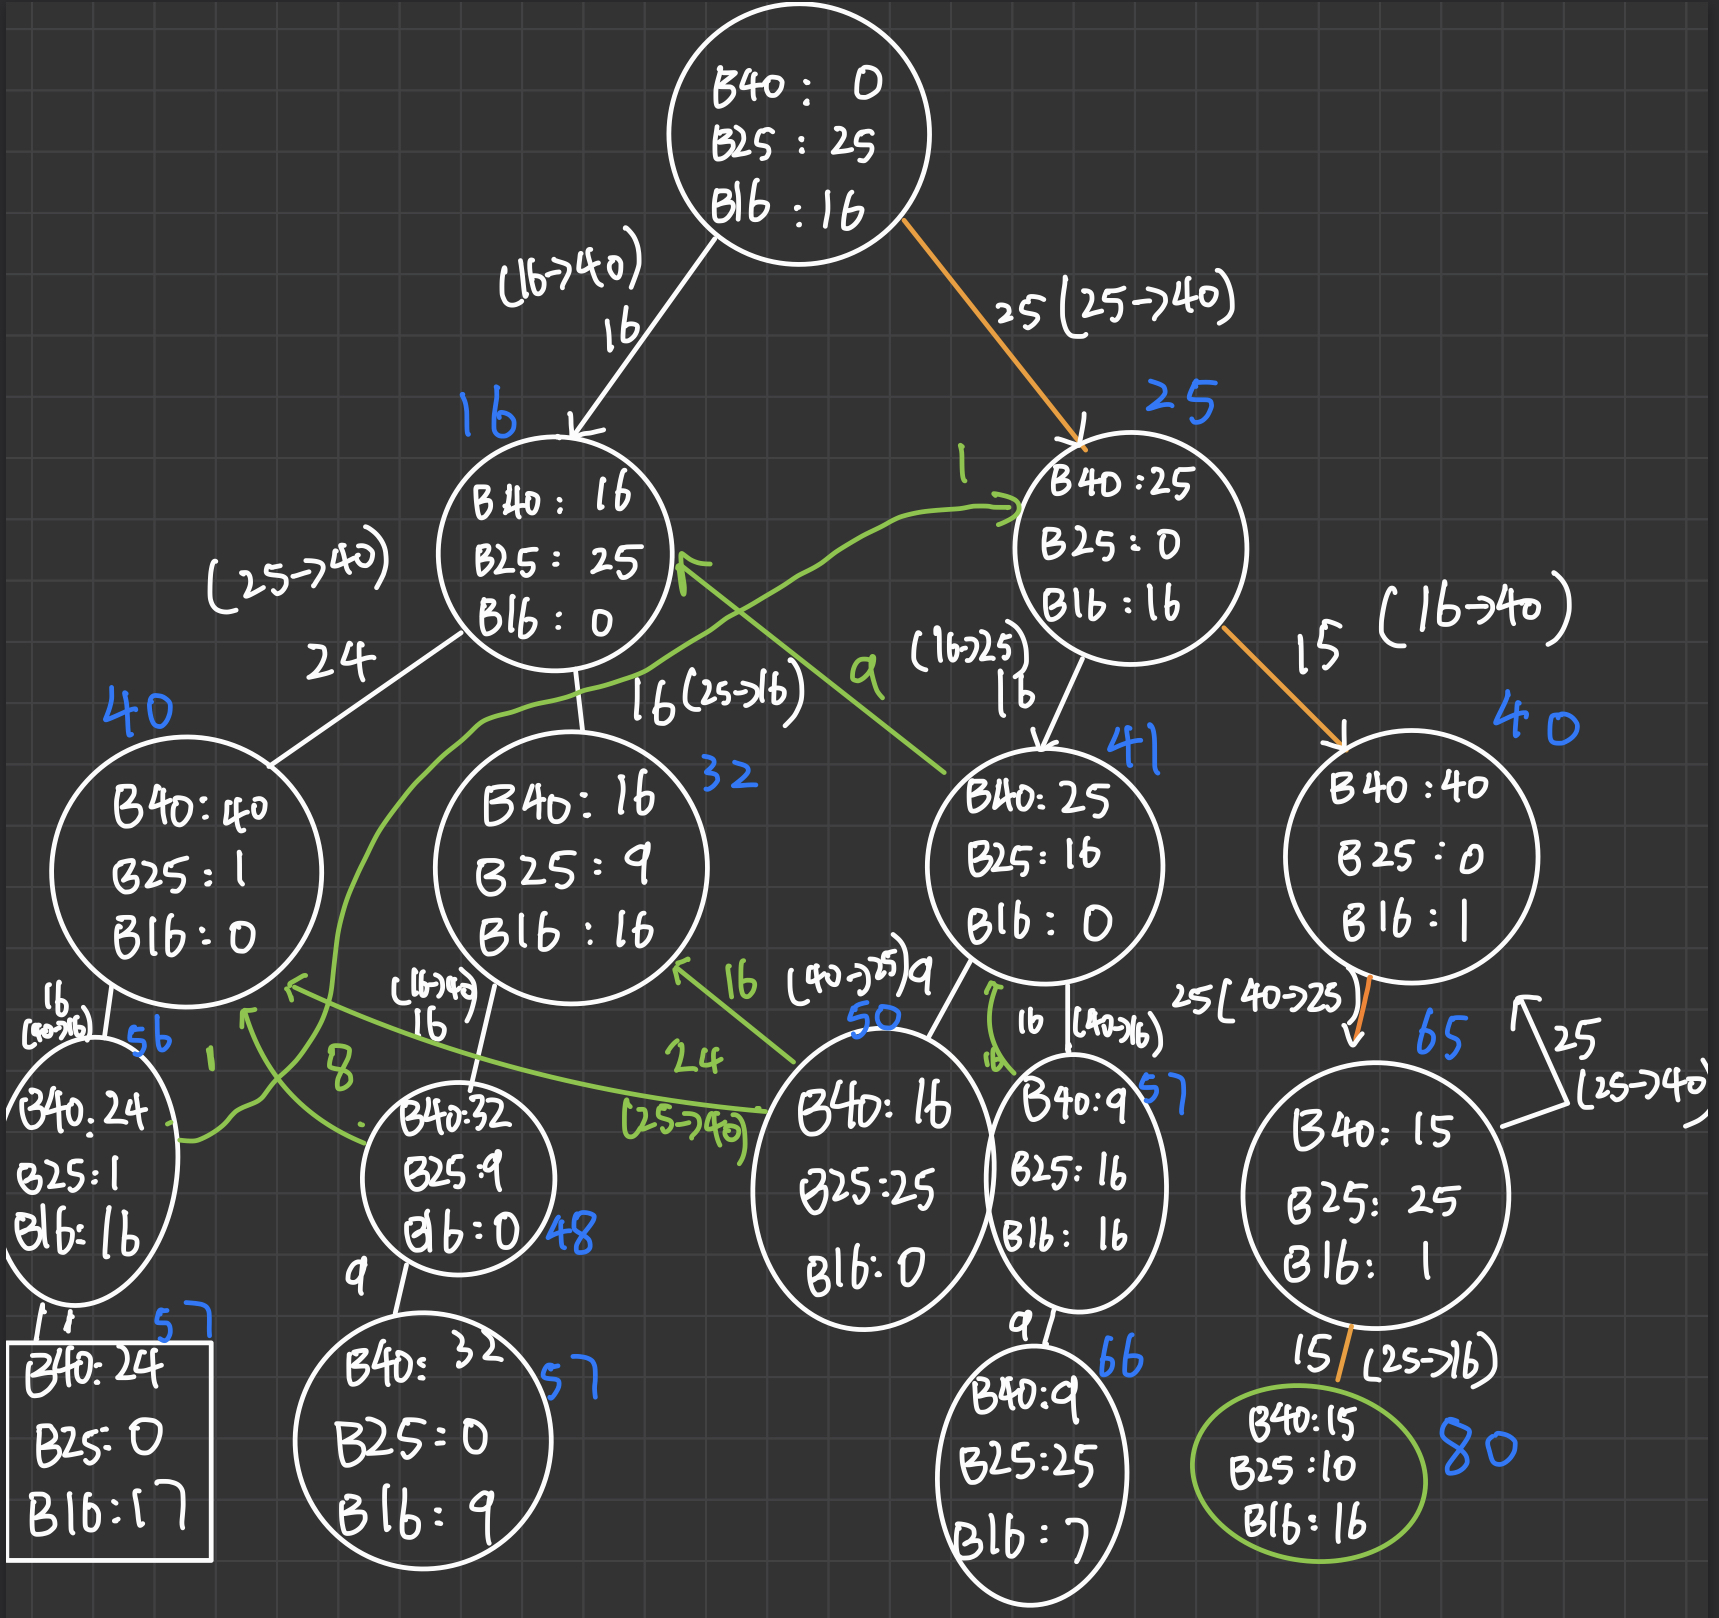
\includegraphics[width=0.7\textwidth]{Q6A.PNG}
\end{center}
\end{proof}

\newpage
\subsubsection{Problem 6\ref{Dijkstra2b}}
\item \label{Dijkstra2b} Clearly describe an algorithm to solve this problem. If you use an algorithm covered in class, it is enough to state that. If you modify an algorithm from class, clearly outline any modifications. Make sure to explicitly specify any parameters that need to be passed to the initial function call.

\begin{proof}[Answer]
\begin{itemize}
\item The key idea to solve this problem is the same as using Dijkstra Algorithm to find the shortest path from source vertex to a target vertex.
\item This algorithm require the Graph G is connected and has no negative-weight edges. The weighted Graph($V,E, w$) and source Vertex s need to be passed to the initial function call.
\item (1)First, the algorithm will initialize an empty Priority Queue, $Q$. Then, for each vertex in the graph, the algorithm will initialize the $dist$ to be $\infty$, $processed$ to $false$ and $predecessor$ to $NULL$. The first element will be placed in the $Q$ is the source node $s$, as (0,25,16). The distance of $s$ would be 0.
\item Next, the algorithm should create a $While$ loop to iterate until the Priority Queue $Q$ becomes an empty set. Inside the $while$ loop, (2) the algorithm will poll the first element,$current$ from the $Q$ and make it to be processed.
\item Another loop (3)inside the $while$ loop is a $for$ loop, which will iterate each unprocessed neighbor $v$ of $current$. In this $for$ loop, we will check if the $current$ vertex $dist +dist(current,v)$ is less than the $v$ vertex $dist$. (4)If it is less than the v $dist$, the  v{dist} will be updated to the $current$ vertex $dist +dist(current,v)$,$v predecessor$ to $current$, and those information will also updated to the Priority Queue $Q$
If it is not, the $for$ loop will keep iterate until $step(4)$ condition appearing or there is no more unprocessed neighbor vertex $v$. 
\item Repeated $step(2)-(4)$ Until the Priority Queue is an empty set. Then, the algorithm will return the updated Graph,G.
\item The cost of finding this transfer can be found on the $dist$ element of target vertex(that  leaves exactly 10 Ah either in the 25-Ah battery or the 16-Ah battery ). And the path of transfer can be found by back-traversing the $predecessor$ of target vertex.

\end{itemize}
%Your answer goes here
\end{proof}



\newpage
\subsubsection{Problem 6\ref{Dijkstra2c}}
\item \label{Dijkstra2c} Apply that algorithm to the question. Report and justify your answer. Here, justification includes the sequences of vertices visited and the total cost. 

\begin{proof}[Answer]
%Your answer goes here
The sequences of vertices visited
\begin{itemize}
\item \textbf{PQ = [((0,25,16),0) ] }
\item \textbf{PQ = [((16,25,0),16) ,((25,0,16),25)  ] }
\item \textbf{PQ = [((25,0,16),25),((16,9,16),32) ,((40,1,0),40)] }
\item \textbf{PQ = [((16,9,16),32) ,((40,1,0),40),((40,0,1),40),((25,16,0),41)] }
\item \textbf{PQ = [((40,1,0),40),((40,0,1),40),((25,16,0),41),((32,9,0),48)] }
\item \textbf{PQ = [((40,0,1),40),((25,16,0),41),((32,9,0),48),((24,1,16),56)] }
\item \textbf{PQ = [((25,16,0),41),((32,9,0),48),((24,1,16),56),,((15,25,1),65)] }
\item \textbf{PQ = [((32,9,0),48),((24,1,16),56),((15,25,1),65),((16,25,0),50),((9,16,16),57)]}
\item \textbf{PQ = [((24,1,16),56),((15,25,1),65),((16,25,0),50),((9,16,16),57),((32,0,9),57)]}
\item \textbf{PQ = [((15,25,1),65),((16,25,0),50),((9,16,16),57),((32,0,9),57),((24,0,17),57)]}
\item \textbf{PQ = [((16,25,0),50),((9,16,16),57),((32,0,9),57),((24,0,17),57),((15,10,16),80)]}
\item \textbf{PQ = [((9,16,16),57),((32,0,9),57),((24,0,17),57),((15,10,16),80)]}
\item \textbf{PQ = [((32,0,9),57),((24,0,17),57),((15,10,16),80),((9,25,7),66)]}
\item \textbf{PQ = [((24,0,17),57),((15,10,16),80),((9,25,7),66)]}
\item \textbf{PQ = [((15,10,16),80),((9,25,7),66)]}
\item \textbf{PQ = [((9,25,7),66)]}
\item \textbf{PQ = [ ]} Algorithm terminates
\end{itemize}
The total cost to find vertex(15,10,16) = 80Ah\\

After applying the algorithm to the question, the graph can be found below:
\begin{center}
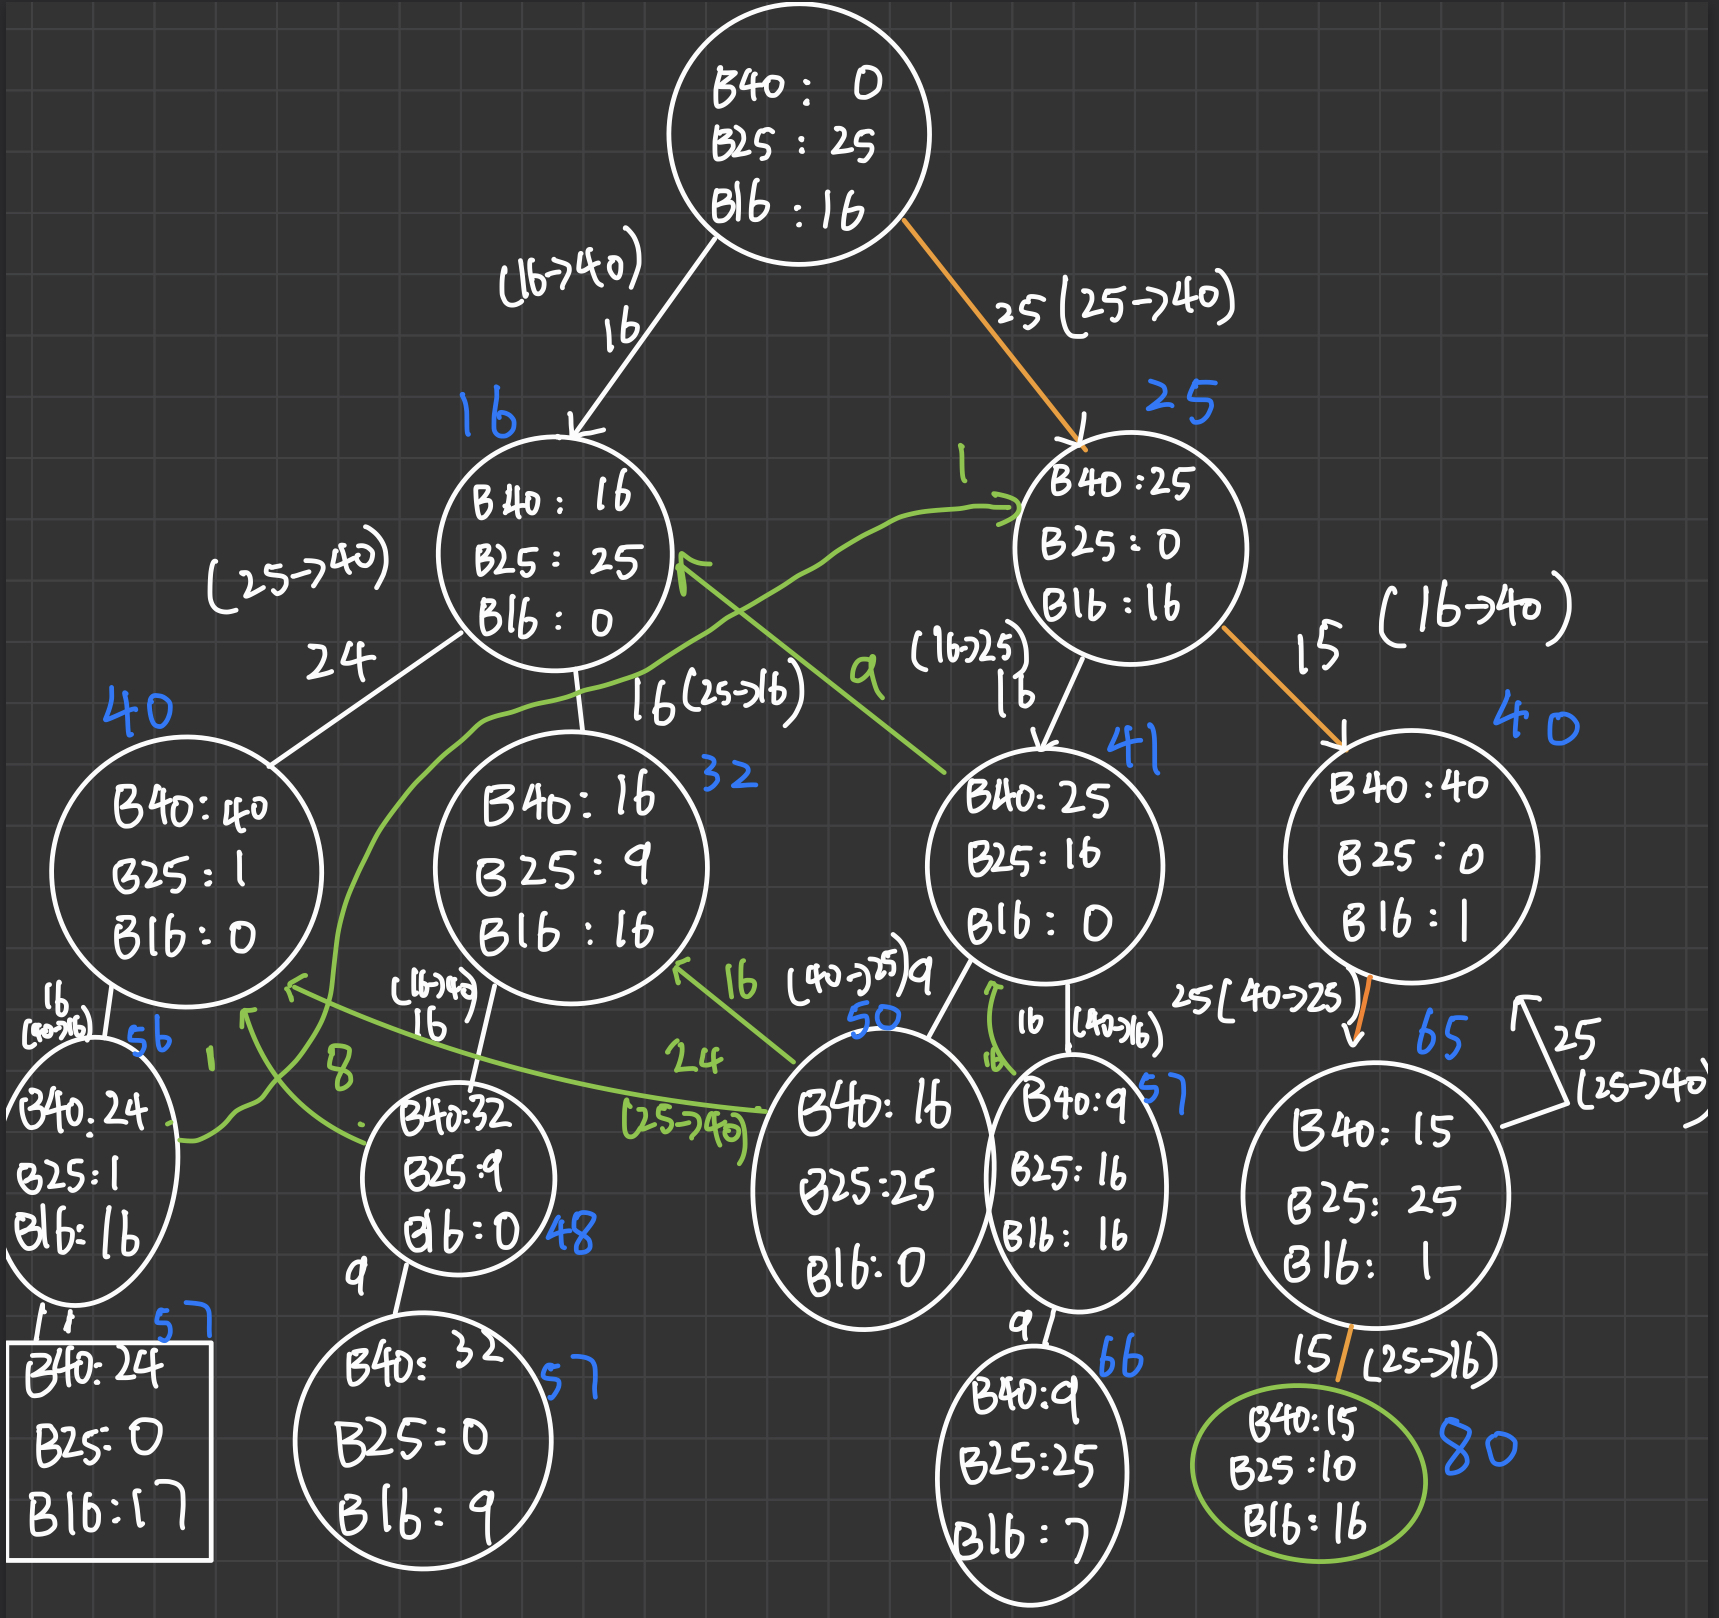
\includegraphics[width=0.7\textwidth]{Q6A.PNG}
\end{center}

\end{proof}

\end{enumerate}
\end{required}



\end{document} % NOTHING AFTER THIS LINE IS PART OF THE DOCUMENT



